% ==========================================================================
%  What if a is A?  --  the lecture notes on analysis of linear systems
%  on one A1 portrait poster.
%  Compile: just   (see justfile; latexmk settings in latexmkrc)
%  Needs: tikz, pgfplots, tcolorbox, cancel, mathpazo (all in TeX Live / MiKTeX)
% ==========================================================================
\RequirePackage{fix-cm}
\documentclass{article}
\usepackage[paperwidth=594mm,paperheight=841mm,left=13mm,right=13mm,top=8mm,bottom=10mm]{geometry}
\usepackage[utf8]{inputenc}
\usepackage[T1]{fontenc}
\usepackage[sc]{mathpazo}          % Palatino text + math
\linespread{1.05}
\usepackage{amsmath,amssymb,bm}
\usepackage{cancel}
\usepackage{xcolor}
\usepackage{tikz}
\usetikzlibrary{arrows.meta,positioning,calc,decorations.pathreplacing,decorations.pathmorphing,decorations.markings,patterns}
\usepackage{pgfplots}
\pgfplotsset{compat=1.16}
\usepackage[most]{tcolorbox}

\pagestyle{empty}
\setlength{\parindent}{0pt}

% ---------------- palette ----------------
\definecolor{paper}{HTML}{F8F5EE}
\definecolor{ink}{HTML}{1E2430}
\definecolor{accent}{HTML}{1F4E79}
\definecolor{accentlt}{HTML}{6E93B5}
\definecolor{trap}{HTML}{9A3B2E}
\definecolor{muted}{HTML}{6B7280}
\definecolor{rule}{HTML}{B9C6D3}
\definecolor{good}{HTML}{3C7A4A}
\pagecolor{paper}
\color{ink}

% ---------------- sizes ----------------
\renewcommand{\normalsize}{\fontsize{13.2}{15.8}\selectfont}
\renewcommand{\small}{\fontsize{11.5}{13.4}\selectfont}
\renewcommand{\footnotesize}{\fontsize{10.8}{12.6}\selectfont}
\newcommand{\eqsize}{\fontsize{14.6}{17.2}\selectfont}
\newcommand{\mathbandsize}{\fontsize{14.6}{17.2}\selectfont}
\normalsize

\newcommand{\setdisplay}{%
  \setlength{\abovedisplayskip}{2pt}\setlength{\belowdisplayskip}{2pt}%
  \setlength{\abovedisplayshortskip}{2pt}\setlength{\belowdisplayshortskip}{2pt}}

% notation: bold for vectors and matrices, as on the blackboard
\newcommand{\A}{\mathbf A}
\newcommand{\B}{\mathbf B}
\newcommand{\Cm}{\mathbf C}
\newcommand{\D}{\mathbf D}
\newcommand{\I}{\mathbf I}
\newcommand{\T}{\mathbf T}
\newcommand{\V}{\mathbf V}
\newcommand{\J}{\mathbf J}
\newcommand{\N}{\mathbf N}
\newcommand{\x}{\mathbf x}
\newcommand{\uu}{\mathbf u}
\newcommand{\y}{\mathbf y}
\newcommand{\vv}{\mathbf v}
\newcommand{\Lam}{\boldsymbol\Lambda}
\newcommand{\ctrb}{\mathcal C}
\newcommand{\obsv}{\mathcal O}
\DeclareMathOperator{\rank}{rank}
\DeclareMathOperator{\tr}{tr}
\DeclareMathOperator{\diag}{diag}

% ---------------- equation group: a thin box holding equations that belong together
\newtcolorbox{eqgroup}[1][]{%
  enhanced, colback=white, colframe=rule, boxrule=0.7pt, arc=2.5mm,
  left=5pt, right=5pt, top=3pt, bottom=0pt, before skip=6pt, after skip=0pt,
  fontupper=\eqsize, before upper={\setdisplay},
  title={#1}, fonttitle=\footnotesize\scshape, coltitle=muted,
  attach boxed title to top left={xshift=4mm, yshift=-\tcboxedtitleheight/2},
  boxed title style={colback=white, colframe=white, boxrule=0pt, arc=0pt,
                     left=3pt, right=3pt, top=0pt, bottom=0pt}}
% short prose inside a box
\newcommand{\note}[1]{{\small\color{muted}#1\par}}

\newcommand{\trapicon}{\tikz[baseline=-0.15em]{%
  \fill[trap, rounded corners=1.2pt] (0,-0.12em) -- (1.15em,-0.12em) -- (0.575em,0.92em) -- cycle;
  \node[white, font=\bfseries\fontsize{11}{11}\selectfont, inner sep=0pt] at (0.575em,0.27em) {!};}}
\newcommand{\trap}[1]{{\centering\fontsize{12.4}{14.6}\selectfont\itshape\color{trap}\trapicon\ #1\par}}

% ---------------- mode box ----------------
% [#1] extra options, #2 index of the eigenvalue, #3 topic (source only), #4 the maxim, #5 unlocks (sits on the bottom border)
\newtcolorbox{mode}[5][]{%
  enhanced, colback=white, colframe=accent, boxrule=1.4pt, arc=4mm,
  left=8pt, right=8pt, top=2pt, bottom=10pt,
  title={%
    \begin{tikzpicture}[baseline=(n.base)]
      \node[rounded corners=6mm, fill=white, text=accent, minimum height=10.5mm, minimum width=11mm, inner xsep=2.2mm, inner ysep=0pt,
            font=\fontsize{25}{25}\selectfont\bfseries] (n) {$\boldsymbol{\lambda_{#2}}$};
    \end{tikzpicture}\hspace{0.5em}%
    {\fontsize{21}{25}\selectfont\bfseries\itshape #4}},% #3 (topic name) kept in the source only, as a label
  colbacktitle=accent, coltitle=white,
  toptitle=1pt, bottomtitle=1pt, lefttitle=6pt, righttitle=10pt,
  segmentation hidden, space to upper, middle=1pt,
  overlay={\node[fill=white, draw=accent, line width=1.4pt, rounded corners=2.5mm,
                 inner xsep=9pt, inner ysep=5pt, font=\small, text=ink, anchor=center]
                 at (frame.south) {#5};},
  #1}

% two-part body: equations left, figure right
\newcommand{\body}[3][0.52]{%
  \begin{minipage}[c]{#1\linewidth}#2\end{minipage}\hfill
  \begin{minipage}[c]{\dimexpr\linewidth-#1\linewidth-6mm\relax}\centering
    \scalebox{\figscale}{\begin{minipage}{\dimexpr\linewidth*100/\figpct\relax}\centering #3\end{minipage}}\end{minipage}\par}
% figure columns are drawn at full size and shrunk uniformly to fit the sheet
\newcommand{\figscale}{0.95}
\newcommand{\figpct}{95}

% common plot style
\pgfplotsset{posterplot/.style={
  width=120mm, height=46mm, axis lines=middle, axis line style={-{Latex[length=3mm]}, thick},
  tick style={draw=none}, ticklabel style={font=\small}, label style={font=\normalsize},
  every axis plot/.append style={line width=1.8pt}}}

% small phase portrait: #1 caption, #2 eigenvalues, #3 drawing in the unit square
\tikzset{traj/.style={accent, line width=1.1pt, postaction={decorate},
  decoration={markings, mark=at position 0.35 with {\arrow{Latex[length=2.2mm]}}}}}
\newcommand{\portrait}[3]{%
  \begin{tikzpicture}[x=12.5mm, y=12.5mm]
    \draw[rule, line width=0.6pt] (-1,-1) rectangle (1,1);
    \begin{scope}
      \clip (-1,-1) rectangle (1,1);
      \draw[muted!50, line width=0.5pt] (-1,0) -- (1,0) (0,-1) -- (0,1);
      #3
    \end{scope}
    \fill[trap] (0,0) circle (0.9mm);
    \node[below=0.6mm, font=\small\bfseries] at (0,-1) {#1};
    \node[below=5.6mm, font=\footnotesize, text=muted] at (0,-1) {#2};
  \end{tikzpicture}}

\begin{document}
% ===================================================================== HEADER
\begin{minipage}[b]{0.60\linewidth}
  {\fontsize{28}{32}\selectfont\scshape\color{muted} Analysis of linear systems, or:}\\[1mm]
  {\fontsize{80}{82}\selectfont\bfseries What if $\boldsymbol{a}$ is $\A$\,?}\\[4mm]
  {\fontsize{36}{42}\selectfont\itshape From $\dot x=ax$ to $\dot{\x}=\A\x+\B\uu$ in ten modes}
\end{minipage}\hfill
\begin{minipage}[b]{0.39\linewidth}\raggedleft
% gutter notes, read top to bottom along the page edges
\begin{tikzpicture}[remember picture, overlay]
  \node[rotate=-90, anchor=center, text=muted, font=\fontsize{14}{17}\selectfont\itshape]
    at ($(current page.east)+(-6.3mm,0mm)$)
    {Guaranteed to be full of errors. Most of them are not LLM hallucinations.};
  \node[rotate=-90, anchor=center, text=muted, font=\fontsize{17}{20}\selectfont\itshape]
    at ($(current page.west)+(6.3mm,0mm)$)
    {A similarity is a translation from Slovene to English: the words (entries) change, the meaning (eigenvalues) does not.};
\end{tikzpicture}%
  {\fontsize{24}{29}\selectfont\color{muted}\itshape
   Ten eigenvalues, all distinct:\\
   the course is diagonalizable, and each mode\\
   may be studied on its own. But they share one $\A$.\\[1mm]
   \upshape\bfseries\color{trap} Cayley--Hamilton to compute,\\ diagonalization to understand.}
\end{minipage}\par
\vspace{2mm}
{\color{accent}\rule{\linewidth}{2.5pt}}
\vspace{2mm}

% ===================================================================== THE SCALAR BAND
\begin{tcolorbox}[enhanced, colback=white, colframe=ink, boxrule=1.6pt, arc=4mm,
  left=10pt, right=10pt, top=4pt, bottom=5pt,
  title={%
    {\fontsize{46}{46}\selectfont\bfseries\itshape A\kern0.02em}%
    {\fontsize{35}{40}\selectfont\bfseries\scshape s simple as $\boldsymbol{\dot x=ax}$}\hfill
    {\fontsize{22}{26}\selectfont\itshape $\A$ is just $a$ with ambitions (and no logarithm).}},
  colbacktitle=ink, coltitle=white, toptitle=4pt, bottomtitle=4pt, lefttitle=10pt, righttitle=14pt]
\mathbandsize\setdisplay
\newcommand{\mathcol}[2][0.327]{\begin{minipage}[t]{#1\linewidth}\vspace{0pt}#2\end{minipage}}
\mathcol[0.245]{%
  \begin{eqgroup}[The substitution that is the whole course]
  \renewcommand{\arraystretch}{1.25}
  \[ \begin{array}{r@{\ \ \longrightarrow\ \ }l}
     e^{at} & e^{\A t}=\Phi(t) \\
     \text{sign of } a & \operatorname{Re}\lambda_i(\A),\ |\lambda_i| \\
     \dfrac{b}{s-a} & \Cm(s\I-\A)^{-1}\B+\D \\[6pt]
     a^k & \A^k \\
     \text{(nothing)} & \rank\ctrb,\ \rank\obsv
  \end{array} \]
  \note{The last row is the only new question: can the input reach, and the output see, \emph{every} state?}
  \end{eqgroup}}\hfill
\mathcol[0.245]{%
  \begin{eqgroup}[The prototype: a capacitor discharging into $R$]
  \[ C\dot x+\frac{x}{R}=0\ \Rightarrow\ \dot x=ax,\quad a=-\frac{1}{RC} \]
  \[ x(t)=x_0\,e^{at}\qquad \tau=RC \]
  \note{$37\,\%$ left after $\tau$, under $1\,\%$ after $5\tau$. With $a>0$ it grows without bound.}
  \end{eqgroup}
  \begin{eqgroup}[Partial fractions: cover up the pole]
  \[ \frac{N(s)}{(s-p_1)(s-p_2)}=\frac{K_1}{s-p_1}+\frac{K_2}{s-p_2} \]
  \[ K_i=(s-p_i)F(s)\big|_{s=p_i} \]
  \note{Repeated pole: add $\frac{K}{(s-p)^2}$, it brings $te^{pt}$.}
  \end{eqgroup}}\hfill
\mathcol[0.245]{%
  \begin{eqgroup}[Laplace: $\tfrac{d}{dt}\to s$]
  \[ \mathcal L\{\dot f\}=sF(s)-f(0) \]
  \renewcommand{\arraystretch}{1.15}
  \[ \begin{array}{c@{\ \leftrightarrow\ }c@{\qquad}c@{\ \leftrightarrow\ }c}
     \delta(t) & 1 & 1(t) & \dfrac1s\\[8pt]
     e^{at} & \dfrac{1}{s-a} & te^{at} & \dfrac{1}{(s-a)^2}\\[8pt]
     \sin\omega t & \dfrac{\omega}{s^2+\omega^2} & \cos\omega t & \dfrac{s}{s^2+\omega^2}
  \end{array} \]
  \end{eqgroup}
  \begin{eqgroup}[The $2\times2$ inverse]
  \[ \begin{bmatrix} a&b\\c&d\end{bmatrix}^{-1}\!\!=\frac{1}{ad-bc}\begin{bmatrix} d&-b\\-c&a\end{bmatrix} \]
  \end{eqgroup}}\hfill
\mathcol[0.245]{%
  \begin{eqgroup}[$Z$: one sample of delay is $z^{-1}$]
  \[ F(z)=\sum_{k\ge0}f[k]\,z^{-k} \]
  \[ f[k-1]\leftrightarrow z^{-1}F \quad f[k+1]\leftrightarrow zF-zf[0] \]
  \renewcommand{\arraystretch}{1.15}
  \[ \begin{array}{c@{\ \leftrightarrow\ }c@{\qquad}c@{\ \leftrightarrow\ }c}
     \delta[k] & 1 & u[k] & \dfrac{z}{z-1}\\[8pt]
     a^k & \dfrac{z}{z-a} & k & \dfrac{z}{(z-1)^2}
  \end{array} \]
  \end{eqgroup}
  \begin{eqgroup}[Euler]
  \[ e^{j\theta}=\cos\theta+j\sin\theta \]
  \end{eqgroup}}

\vspace{6pt}
\trap{Every chapter below is this box with a matrix in place of $a$. What breaks is division and the logarithm: there is no $\frac{d\x}{\x}$. What survives is the answer $\x(t)=e^{\A t}\x_0$, once $e^{\A t}$ means something.}
\end{tcolorbox}

\vspace{6mm}

% ===================================================================== THE TEN MODES
\noindent\begin{minipage}[t]{0.488\linewidth}
\begin{mode}[equal height group=row1]{1}{LTI}{Add the inputs, add the outputs.}{Unlocks: impulse response, convolution, $e^{\A t}$, transfer functions: every other box on this sheet.}
\body{%
  \begin{eqgroup}[Linear: superposition]
  \[ L(au_1+bu_2)=a\,L(u_1)+b\,L(u_2) \]
  \end{eqgroup}
  \begin{eqgroup}[Time-invariant: a delay in is a delay out]
  \[ u(t-\tau)\ \mapsto\ y(t-\tau)\quad\forall\tau \]
  \end{eqgroup}
  \vspace{2mm}
  \note{\textbf{Breaks linearity:} $yu$, $y^2$, $e^y$, $\sin u$, $\sqrt y$, and a constant offset ($y=\alpha u+\beta$ is affine). \textbf{Breaks time invariance:} an explicit $t$ in a coefficient or forcing. \textbf{Also required:} lumped (finitely many states, no PDE, no delay; circuits while $d<\lambda/20$) and deterministic (no noise).}}%
{%
  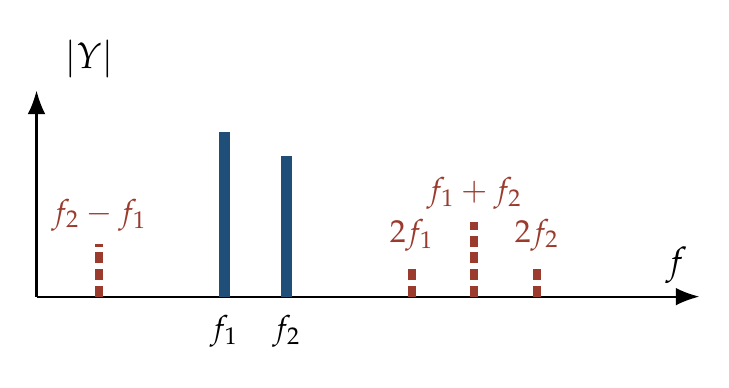
\begin{tikzpicture}
  \begin{axis}[posterplot, width=100mm, height=42mm, clip=false, xmin=0, xmax=10.6, ymin=0, ymax=1.25,
      xlabel={$f$}, ylabel={$|Y|$}, xtick={3,4}, xticklabels={$f_1$,$f_2$}, ytick=\empty,
      every axis y label/.style={at={(axis description cs:0,1)}, anchor=south west, xshift=2mm}]
    \draw[accent, line width=4pt] (axis cs:3,0) -- (axis cs:3,1);
    \draw[accent, line width=4pt] (axis cs:4,0) -- (axis cs:4,0.85);
    \draw[trap, line width=3pt, dash pattern=on 4pt off 2pt] (axis cs:1,0) -- (axis cs:1,0.32);
    \draw[trap, line width=3pt, dash pattern=on 4pt off 2pt] (axis cs:6,0) -- (axis cs:6,0.2);
    \draw[trap, line width=3pt, dash pattern=on 4pt off 2pt] (axis cs:7,0) -- (axis cs:7,0.45);
    \draw[trap, line width=3pt, dash pattern=on 4pt off 2pt] (axis cs:8,0) -- (axis cs:8,0.2);
    \node[trap, font=\small, above] at (axis cs:1,0.32) {$f_2-f_1$};
    \node[trap, font=\small, above] at (axis cs:7,0.45) {$f_1+f_2$};
    \node[trap, font=\small, above] at (axis cs:6,0.2) {$2f_1$};
    \node[trap, font=\small, above] at (axis cs:8,0.2) {$2f_2$};
  \end{axis}
  \end{tikzpicture}\\[1mm]
  {\small\color{muted}On the bench: two tones in. An LTI box returns only $f_1$ and $f_2$, rescaled and phase-shifted. Every other line is nonlinearity. A test can disprove linearity, never prove it.}}
\tcblower
\trap{$\dot y=5y+4t$ is linear but time-varying; $y=\alpha u+\beta$ is time-invariant but not linear. Check the two separately.}
\end{mode}
\end{minipage}\hfill%
\begin{minipage}[t]{0.488\linewidth}
\begin{mode}[equal height group=row1]{2}{Modeling}{One state per energy store.}{Unlocks: $\dot\x=\A\x+\B\uu$ for circuits, cars, motors, populations and economies.}
\body{%
  \begin{eqgroup}[Pick the states: what cannot jump]
  \[ L\to i_L \quad C\to v_C \quad m\to x,\,v \quad J\to\theta,\,\omega \]
  \end{eqgroup}
  \begin{eqgroup}[The parentheses hold every sign]
  \[ F_k=k\,(x_{\text{other}}-x_{\text{self}}) \quad F_b=b\,(\dot x_{\text{other}}-\dot x_{\text{self}}) \]
  \end{eqgroup}
  \begin{eqgroup}[$n$-th order ODE $\to$ companion form]
  \[ x_1=y,\ x_2=\dot y,\ \dots \quad \A=\begin{bmatrix} 0&1&0\\0&0&1\\-a_0&-a_1&-a_2\end{bmatrix} \]
  \end{eqgroup}
  \vspace{2mm}
  \note{\textbf{Circuits:} ground a voltage-source terminal; a floating source needs a supernode. Start from $C\dot v_C=i_C$ and $L\dot i_L=v_L$, use the node equations only to fill in. \textbf{Analogy:} $m\leftrightarrow L$, $k\leftrightarrow 1/C$, $b\leftrightarrow R$.}}%
{%
  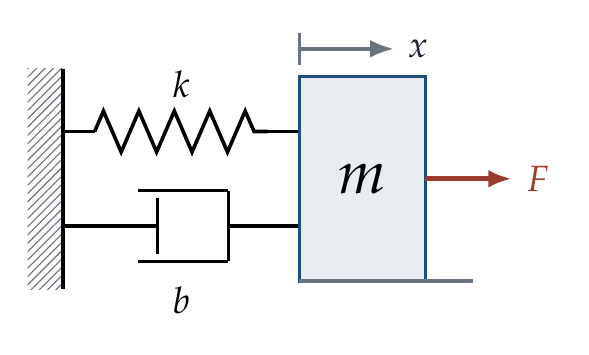
\begin{tikzpicture}[line width=1.3pt, >={Latex[length=3mm]}]
    % wall
    \fill[pattern=north east lines, pattern color=muted] (-0.45,-0.2) rectangle (0,2.6);
    \draw (0,-0.2) -- (0,2.6);
    % spring
    \draw (0,1.8) -- (0.4,1.8);
    \draw[decorate, decoration={zigzag, segment length=4.5mm, amplitude=2.6mm}] (0.4,1.8) -- (2.6,1.8);
    \draw (2.6,1.8) -- (3.0,1.8);
    \node[above=2.5mm] at (1.5,1.8) {$k$};
    % damper
    \draw (0,0.6) -- (1.2,0.6);
    \draw (1.2,0.25) -- (1.2,0.95);
    \draw (0.95,0.15) -- (2.1,0.15) (0.95,1.05) -- (2.1,1.05) (2.1,0.15) -- (2.1,1.05);
    \draw (2.1,0.6) -- (3.0,0.6);
    \node[below=1.5mm] at (1.5,0.15) {$b$};
    % mass
    \draw[fill=accent!10, draw=accent] (3.0,-0.1) rectangle (4.6,2.5);
    \node[font=\fontsize{22}{22}\selectfont] at (3.8,1.2) {$m$};
    % force and coordinate
    \draw[->, trap, line width=1.8pt] (4.6,1.2) -- (5.7,1.2) node[right]{$F$};
    \draw[->, muted] (3.0,2.85) -- (4.2,2.85) node[right, text=ink]{$x$};
    \draw[muted] (3.0,2.65) -- (3.0,3.05);
    % ground line
    \draw[muted] (3.0,-0.1) -- (5.2,-0.1);
  \end{tikzpicture}\\[2mm]
  {\eqsize $m\ddot x+b\dot x+kx=F$}\\[2mm]
  {\fontsize{16}{20}\selectfont
  $\displaystyle\frac{d}{dt}\begin{bmatrix} x\\ v\end{bmatrix}=\begin{bmatrix} 0&1\\-\dfrac km&-\dfrac bm\end{bmatrix}\begin{bmatrix} x\\ v\end{bmatrix}+\begin{bmatrix} 0\\ \dfrac1m\end{bmatrix}F$}\\[2mm]
  {\small\color{muted}Sanity: at rest the springs carry the static load. In circuits: $\A$'s diagonal negative, its off-diagonals of opposite sign ($L$ and $C$ trade energy).}}
\tcblower
\trap{$\Cm$ and $\D$ are constant: no derivative may appear in the output equation. $v_L=L\,\dot i_L$ is a state equation in disguise.}
\end{mode}
\end{minipage}

\vspace{3mm plus 1fill}

\noindent\begin{minipage}[t]{0.488\linewidth}
\begin{mode}[equal height group=row2]{3}{Linear algebra}{Same map, different words.}{Unlocks: modes, decoupling, $e^{\A t}$ and $\A^k$, and every rank test in $\lambda_7$.}
\body[0.55]{%
  \begin{eqgroup}[Eigenvalues, eigenvectors, multiplicities]
  \[ \det(\A-\lambda\I)=0 \qquad (\A-\lambda\I)\,\vv=\mathbf 0 \]
  \[ m_g=n-\rank(\A-\lambda\I)\qquad 1\le m_g\le m_a \]
  \end{eqgroup}
  \begin{eqgroup}[Similarity keeps the meaning]
  \[ \tilde\A=\T^{-1}\A\T \qquad f(\A)=\T f(\tilde\A)\,\T^{-1} \]
  \[ \det\A=\textstyle\prod\lambda_i\qquad \tr\A=\sum\lambda_i \]
  \[ \A=\V\Lam\V^{-1}\ \ \text{iff } m_g=m_a\ \text{for every }\lambda \]
  \end{eqgroup}
  \begin{eqgroup}[Jordan: as diagonal as it gets]
  \[ \J_k(\lambda)=\begin{bmatrix}\lambda&1&\\&\lambda&1\\&&\lambda\end{bmatrix}\quad
     \begin{array}{l}\#\text{blocks}=m_g\\ \textstyle\sum\text{sizes}=m_a\end{array} \]
  \[ (\A-\lambda\I)\vv_j=\vv_{j-1},\ \ \text{chain built from the top} \]
  \end{eqgroup}}%
{%
  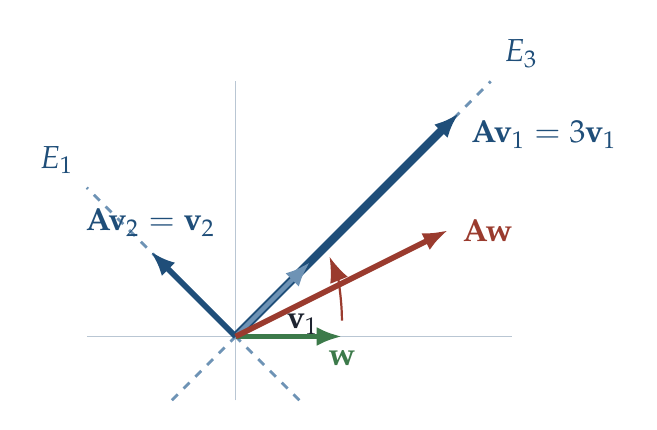
\begin{tikzpicture}[x=13.5mm, y=13.5mm, >={Latex[length=3.2mm]}]
    \draw[rule, line width=0.6pt] (-1.4,0) -- (2.6,0) (0,-0.6) -- (0,2.4);
    \draw[accentlt, dashed, line width=1pt] (-0.6,-0.6) -- (2.4,2.4) node[above right, font=\small, text=accent]{$E_3$};
    \draw[accentlt, dashed, line width=1pt] (0.6,-0.6) -- (-1.4,1.4) node[above left, font=\small, text=accent]{$E_1$};
    % eigenvector stretched x3
    \draw[->, accent, line width=3pt] (0,0) -- (2.1,2.1);
    \draw[->, accentlt, line width=1.6pt] (0,0) -- (0.7,0.7) node[midway, below right, font=\small, text=ink]{$\vv_1$};
    \node[accent, font=\small, right] at (2.1,1.9) {$\A\vv_1=3\vv_1$};
    % eigenvector x1
    \draw[->, accent, line width=2pt] (0,0) -- (-0.8,0.8) node[above, font=\small]{$\A\vv_2=\vv_2$};
    % knocked off
    \draw[->, good, line width=1.6pt] (0,0) -- (1,0) node[below, font=\small]{$\mathbf w$};
    \draw[->, trap, line width=2pt] (0,0) -- (2,1) node[right, font=\small]{$\A\mathbf w$};
    \draw[trap, line width=0.8pt, ->] (1.0,0.15) arc[start angle=0, end angle=22, radius=1.6];
  \end{tikzpicture}\\[1mm]
  {\eqsize $\A=\begin{bmatrix}2&1\\1&2\end{bmatrix}\ \overset{\T\,=\,[\vv_1\ \vv_2]}{\longrightarrow}\ \tilde\A=\begin{bmatrix}3&0\\0&1\end{bmatrix}$}\\[2mm]
  {\small\color{muted}On its eigenlines $\A$ only stretches; everything else it also turns. In the eigenbasis the off-diagonal 1s vanish: they belonged to the coordinates, not to the map.}\\[2mm]
  {\small\color{muted}Defective ($m_g<m_a$): no $\V$ exists. Block sizes from ranks: $\#\{\text{size}\ge k\}=\rank\N^{k-1}-\rank\N^k$, with $\N=\A-\lambda\I$.}}
\tcblower
\trap{The rows of $\A-\lambda\I$ are \emph{supposed} to be dependent: that is what makes $\lambda$ an eigenvalue. A zero row is good news, not an error.}
\end{mode}
\end{minipage}\hfill%
\begin{minipage}[t]{0.488\linewidth}
\begin{mode}[equal height group=row2]{4}{State-space solution}{The state forgets nothing it needs.}{Unlocks: step and impulse responses, sampling ($\A_D=e^{\A_cT}$), the controllability proof, observers.}
\body[0.56]{%
  \begin{eqgroup}[The whole solution, in one line]
  \[ \x(t)=\underbrace{e^{\A(t-t_0)}\x(t_0)}_{\text{free: initial state}}+\underbrace{\int_{t_0}^{t}e^{\A(t-\tau)}\B\uu(\tau)\,d\tau}_{\text{forced: convolution}} \]
  \end{eqgroup}
  \begin{eqgroup}[$\Phi(t)=e^{\A t}$, the state-transition matrix]
  \[ \Phi(0)=\I\qquad \Phi(t_1+t_2)=\Phi(t_1)\Phi(t_2) \]
  \[ \Phi^{-1}(t)=\Phi(-t)\qquad \dot\Phi=\A\Phi=\Phi\A \]
  \end{eqgroup}
  \begin{eqgroup}[Impulse response and the final value]
  \[ h(t)=\Cm\Phi(t)\B+\D\,\delta(t)\qquad y=h*u \]
  \[ \x(\infty)=-\A^{-1}\B\,u\quad(\text{stable, constant }u) \]
  \end{eqgroup}}%
{%
  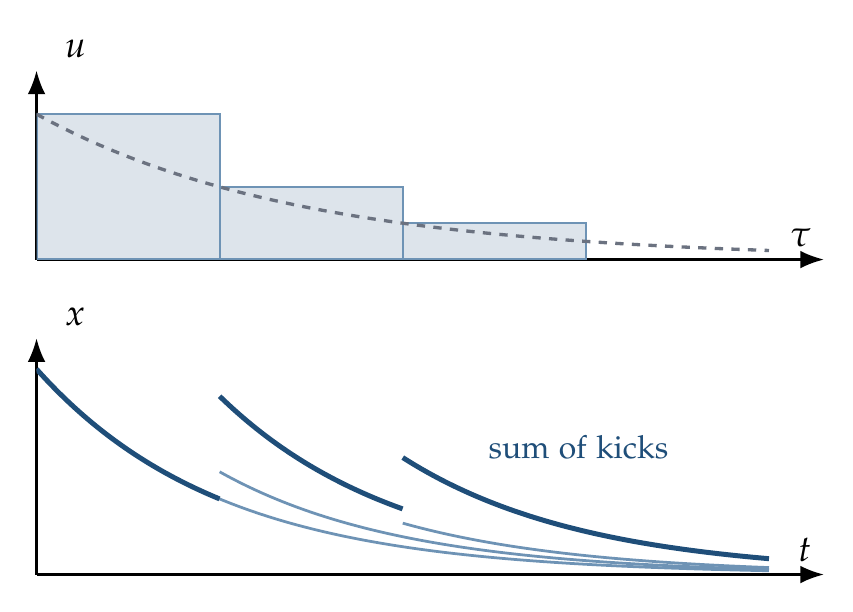
\begin{tikzpicture}
  \begin{axis}[posterplot, width=100mm, height=24mm, scale only axis, xmin=0, xmax=4.3, ymin=0, ymax=1.3,
      xlabel={$\tau$}, ylabel={$u$}, xtick=\empty, ytick=\empty, name=uu,
      every axis y label/.style={at={(axis description cs:0,1)}, anchor=south west, xshift=2mm}]
    \fill[accent!15] (axis cs:0,0) rectangle (axis cs:1,1);
    \fill[accent!15] (axis cs:1,0) rectangle (axis cs:2,0.5);
    \fill[accent!15] (axis cs:2,0) rectangle (axis cs:3,0.25);
    \draw[accentlt, line width=0.8pt] (axis cs:0,0) rectangle (axis cs:1,1) (axis cs:1,0) rectangle (axis cs:2,0.5) (axis cs:2,0) rectangle (axis cs:3,0.25);
    \addplot[muted, dashed, domain=0:4, samples=60, line width=1.2pt] {2^(-x)};
  \end{axis}
  \begin{axis}[posterplot, at={(uu.south west)}, anchor=north west, yshift=-10mm, width=100mm, height=30mm, scale only axis,
      xmin=0, xmax=4.3, ymin=0, ymax=1.15, xlabel={$t$}, ylabel={$x$}, xtick=\empty, ytick=\empty,
      every axis y label/.style={at={(axis description cs:0,1)}, anchor=south west, xshift=2mm}]
    \addplot[accentlt, domain=0:4, samples=80, line width=1pt] {exp(-x)};
    \addplot[accentlt, domain=1:4, samples=80, line width=1pt] {0.5*exp(-(x-1))};
    \addplot[accentlt, domain=2:4, samples=80, line width=1pt] {0.25*exp(-(x-2))};
    \addplot[accent, domain=0:0.999, samples=40] {exp(-x)};
    \addplot[accent, domain=1:1.999, samples=40] {exp(-x)+0.5*exp(-(x-1))};
    \addplot[accent, domain=2:4, samples=60] {exp(-x)+0.5*exp(-(x-1))+0.25*exp(-(x-2))};
    \node[accent, font=\small, anchor=west] at (axis cs:2.4,0.62) {sum of kicks};
  \end{axis}
  \end{tikzpicture}\\[1mm]
  {\small\color{muted}Slice the input into kicks $u(\tau)\,d\tau$. Each one lands through $\B$ and evolves freely for $t-\tau$. Linearity adds the responses; time invariance makes them all the same shape. That sum is the convolution.}}
\tcblower
\trap{The integral starts at $t_0$, where knowledge of the input starts. Start it at $0$ when the experiment began elsewhere and terms go missing.}
\end{mode}
\end{minipage}

\vspace{3mm plus 1fill}

\noindent\begin{minipage}[t]{0.488\linewidth}
\begin{mode}[equal height group=row3]{5}{Phi}{Four ways to skin a cat.}{At the end, the same dead cat: $\dot\Phi=\A\Phi$, $\Phi(0)=\I$ has exactly one solution.}
\body[0.53]{%
  \begin{eqgroup}[Taylor: the definition]
  \[ e^{\A t}=\sum_{k=0}^{\infty}\frac{(\A t)^k}{k!}=\I+\A t+\frac{(\A t)^2}{2!}+\cdots \]
  \end{eqgroup}
  \begin{eqgroup}[Laplace: invert the resolvent]
  \[ \Phi(t)=\mathcal L^{-1}\big\{(s\I-\A)^{-1}\big\} \]
  \end{eqgroup}
  \begin{eqgroup}[Diagonalize, or Jordan]
  \[ \Phi=\V\,\diag\!\big(e^{\lambda_it}\big)\,\V^{-1}\qquad \Phi=\T\,e^{\J t}\,\T^{-1} \]
  \end{eqgroup}
  \begin{eqgroup}[Cayley--Hamilton: $g(\A)=\mathbf 0$]
  \[ e^{\A t}=\sum_{i=0}^{n-1}\alpha_i(t)\,\A^i\qquad e^{\lambda_jt}=\sum_{i=0}^{n-1}\alpha_i(t)\,\lambda_j^i \]
  \note{Repeated $\lambda$: differentiate the scalar equation $\tfrac{d}{d\lambda}$, which supplies the $te^{\lambda t}$. Works for any analytic $f$, any $\A$, no eigenvectors.}
  \end{eqgroup}}%
{%
  {\fontsize{17}{21}\selectfont
  $\displaystyle e^{\J_4(\lambda)t}=e^{\lambda t}\!\begin{bmatrix}
    1 & \textcolor{accent}{t} & \textcolor{good}{\frac{t^2}{2!}} & \textcolor{trap}{\frac{t^3}{3!}}\\[3pt]
    0 & 1 & \textcolor{accent}{t} & \textcolor{good}{\frac{t^2}{2!}}\\[3pt]
    0 & 0 & 1 & \textcolor{accent}{t}\\[3pt]
    0 & 0 & 0 & 1\end{bmatrix}$}\\[3mm]
  {\small\color{muted}$\J_k=\lambda\I+\N$ with $\N^k=\mathbf 0$ (nilpotent), so the series stops. Powers of $t$ climb the superdiagonals: a $k\times k$ block reaches $t^{k-1}e^{\lambda t}$. They come from the 1s, not from repetition alone.}\\[4mm]
  \renewcommand{\arraystretch}{1.25}
  {\small\begin{tabular}{@{}l@{\ \ }l@{}}
    \textbf{Taylor} & general, tedious\\
    \textbf{Laplace} & neat, needs symbolic algebra\\
    \textbf{Diag./Jordan} & shows the modes; defective $\A$ is laborious\\
    \textbf{C--H} & computes anything, explains nothing
  \end{tabular}}}
\tcblower
\trap{In Cayley--Hamilton, differentiate with respect to $\lambda$, not $t$. Whatever the route, check $\Phi(0)=\I$ and $\dot\Phi(0)=\A$.}
\end{mode}
\end{minipage}\hfill%
\begin{minipage}[t]{0.488\linewidth}
\begin{mode}[equal height group=row3]{6}{Stability}{Left of the axis, all is well.}{Unlocks: BIBO, robustness margins, pole placement, local stability of nonlinear systems ($\lambda_9$).}
\body[0.50]{%
  \begin{eqgroup}[Lyapunov, read off the eigenvalues of $\A$]
  \renewcommand{\arraystretch}{1.3}
  \[ \begin{array}{l@{\ \Rightarrow\ }l}
    \text{all }\operatorname{Re}\lambda_i<0 & \text{asymptotically stable}\\
    \text{all }\operatorname{Re}\lambda_i\le0\,^{*} & \text{marginally stable}\\
    \text{any }\operatorname{Re}\lambda_i>0 & \text{unstable}
  \end{array} \]
  \note{$^{*}$Eigenvalues on the axis must be simple; precisely: only $1\times1$ Jordan blocks there. The double integrator $\ddot x=0$ has $\lambda=0$ twice in one block and drifts as $x_0+\dot x_0t$.}
  \end{eqgroup}
  \begin{eqgroup}[BIBO: only the poles of $G(s)$ count]
  \[ \text{all poles of }G(s)\text{ in }\operatorname{Re}s<0 \]
  \note{Asymptotic $\Rightarrow$ BIBO; the converse only for a minimal realization. A hidden unstable mode can sit behind a perfectly BIBO-stable $G(s)$. Hidden but decaying is fine: \emph{stabilizable}, \emph{detectable}.}
  \end{eqgroup}}%
{%
  \portrait{node}{$\lambda=-1,\,-3$}{%
    \foreach \a/\b in {1/1,-1/1,1/-1,-1/-1,0.35/1,-0.35/1,0.35/-1,-0.35/-1,1/0.4,-1/0.4,1/-0.4,-1/-0.4}
      \draw[traj] plot[domain=0:2, samples=25] ({\a*exp(-\x)},{\b*exp(-3*\x)});}\hspace{4mm}%
  \portrait{saddle}{$\lambda=+1,\,-1$}{%
    \foreach \a/\b in {0.08/1,-0.08/1,0.08/-1,-0.08/-1,0.3/1,-0.3/1,0.3/-1,-0.3/-1}
      \draw[traj] plot[domain=0:2.6, samples=25] ({\a*exp(\x)},{\b*exp(-\x)});
    \draw[traj] (0,1) -- (0,0.02); \draw[traj] (0,-1) -- (0,-0.02);
    \draw[traj] (0.02,0) -- (1,0); \draw[traj] (-0.02,0) -- (-1,0);}\\[3mm]
  \portrait{focus}{$\lambda=-0.15\pm1.6j$}{%
    \draw[traj] plot[domain=0:16, samples=200] ({0.98*exp(-0.15*\x)*cos(deg(1.6*\x))},{0.75*exp(-0.15*\x)*sin(deg(1.6*\x))});}\hspace{4mm}%
  \portrait{center}{$\lambda=\pm j\omega$}{%
    \foreach \r in {0.3,0.6,0.9}
      \draw[accent, line width=1.1pt, postaction={decorate}, decoration={markings, mark=at position 0.25 with {\arrow{Latex[length=2.2mm]}}}] (0,0) ellipse[x radius=\r, y radius=0.8*\r];}\\[2mm]
  {\small\color{muted}Near an equilibrium the eigenvalues set the picture: real, same sign: node; opposite signs: saddle; complex: focus; on the axis: center.}}
\tcblower
\trap{Marginal stability is fragile: a nudge to $\A$ tips it either way. Asymptotic stability has a margin: the distance to the axis.}
\end{mode}
\end{minipage}

\vspace{3mm plus 1fill}

\noindent\begin{minipage}[t]{0.488\linewidth}
\begin{mode}[equal height group=row4]{7}{Controllability and observability}{Can you push it? Can you see it?}{Unlocks: state feedback $\uu=-K\x$, observers and the Kalman filter, minimal realizations.}
\body[0.52]{%
  \begin{eqgroup}[Controllable: only $(\A,\B)$ matter]
  \[ \ctrb=\begin{bmatrix}\B&\A\B&\cdots&\A^{n-1}\B\end{bmatrix}\qquad \rank\ctrb=n \]
  \end{eqgroup}
  \begin{eqgroup}[Observable: only $(\A,\Cm)$ matter; it is the dual]
  \[ \obsv^{\mathsf T}=\begin{bmatrix}\Cm^{\mathsf T}&\A^{\mathsf T}\Cm^{\mathsf T}&\cdots&(\A^{\mathsf T})^{n-1}\Cm^{\mathsf T}\end{bmatrix}\qquad \rank\obsv=n \]
  \note{$\obsv$ stacks $\Cm,\ \Cm\A,\ \dots,\ \Cm\A^{n-1}$ as rows: $(\A,\Cm)$ is observable iff $(\A^{\mathsf T},\Cm^{\mathsf T})$ is controllable.}
  \end{eqgroup}
  \begin{eqgroup}[Why it stops at $n-1$: Cayley--Hamilton]
  \[ \x(t)=\textstyle\sum_{k<n}\A^k\B\,\mathbf w_k=\ctrb\,\mathbf w \]
  \note{Reachable states live in the range of $\ctrb$. One input cannot control two Jordan blocks of the same $\lambda$: you need $m\ge\max_i m_{g,i}$ inputs.}
  \end{eqgroup}}%
{%
  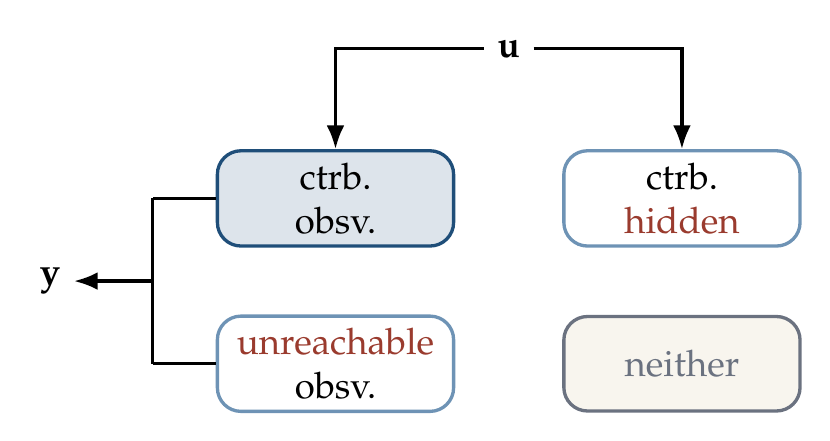
\begin{tikzpicture}[>={Latex[length=3mm]}, line width=1.2pt,
     sub/.style={draw, rounded corners=3mm, minimum width=30mm, minimum height=12mm, align=center, font=\normalsize}]
    \node[sub, fill=accent!15, draw=accent] (co) at (0,0) {ctrb.\\ obsv.};
    \node[sub, fill=white, draw=accentlt] (cn) at (4.4,0) {ctrb.\\ \textcolor{trap}{hidden}};
    \node[sub, fill=white, draw=accentlt] (no) at (0,-2.1) {\textcolor{trap}{unreachable}\\ obsv.};
    \node[sub, fill=paper, draw=muted, text=muted] (nn) at (4.4,-2.1) {neither};
    \node (u) at (2.2,1.9) {$\uu$};
    \draw[->] (u) -| (co.north);
    \draw[->] (u) -| (cn.north);
    \draw (co.west) -- ++(-0.8,0) coordinate (a);
    \draw (no.west) -- ++(-0.8,0) coordinate (b);
    \draw (a) -- (b);
    \draw[->] ($(a)!0.5!(b)$) -- ++(-1.0,0) node[left]{$\y$};
  \end{tikzpicture}\\[2mm]
  {\small\color{muted}Kalman's four rooms. Only the top-left one reaches $G(s)$; the others leave as cancelling pole--zero pairs:}\\[2mm]
  {\eqsize $\displaystyle G(s)=\frac{\xcancel{(s+1)}(s+4)}{\xcancel{(s+1)}(s+2)(s+3)}$}\\[1mm]
  {\small\color{muted}Here $\Cm\vv=0$ for the eigenvector of $\lambda=-1$: the sensor never sees that mode.}}
\tcblower
\trap{Test the rank, not the determinant: $\ctrb$ is $n\times nm$, square only for one input. A zero row of $\B$ in modal form is a mode the input never touches.}
\end{mode}
\end{minipage}\hfill%
\begin{minipage}[t]{0.488\linewidth}
\begin{mode}[equal height group=row4]{8}{Transfer functions}{Convolution becomes multiplication.}{Unlocks: frequency response $G(j\omega)$, Bode and Nyquist, filters, PID, block-diagram algebra.}
\body[0.54]{%
  \begin{eqgroup}[From state space (zero initial state)]
  \[ \mathbf G(s)=\Cm(s\I-\A)^{-1}\B+\D \]
  \[ \text{poles}=\operatorname{eig}\A\ \ (\text{if minimal})\qquad h=\mathcal L^{-1}\{G\} \]
  \end{eqgroup}
  \begin{eqgroup}[From the ODE: $\tfrac{d}{dt}\to s$, zero initial conditions]
  \[ G(s)=\frac{Y}{U}=\frac{b_ms^m+\cdots+b_0}{a_ns^n+\cdots+a_0} \]
  \end{eqgroup}
  \begin{eqgroup}[Block algebra, and two free sanity checks]
  \[ \underset{\text{series}}{G_1G_2}\qquad \underset{\text{parallel}}{G_1+G_2}\qquad \underset{\text{feedback}}{\frac{G}{1+GH}} \]
  \[ h(0^+)=\lim_{s\to\infty}sG(s)\qquad \int_0^\infty h\,dt=G(0) \]
  \end{eqgroup}}%
{%
  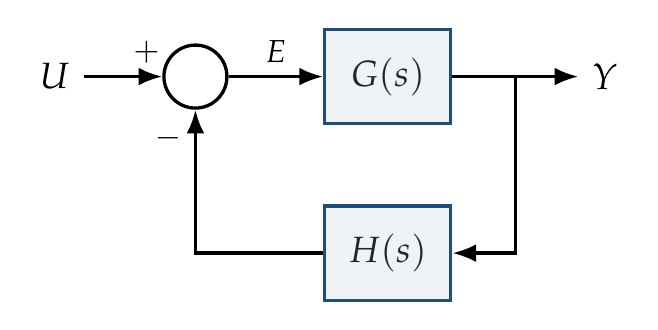
\begin{tikzpicture}[>={Latex[length=3mm]}, line width=1.2pt,
     blk/.style={draw, accent, fill=accent!7, minimum width=16mm, minimum height=12mm, font=\normalsize, text=ink},
     sum/.style={draw, circle, minimum size=8mm, inner sep=0pt, font=\small}]
    \node (u) {$U$};
    \node[sum, right=10mm of u] (s) {};
    \node[blk, right=12mm of s] (G) {$G(s)$};
    \node[right=16mm of G] (y) {$Y$};
    \node[blk, below=10mm of G] (H) {$H(s)$};
    \draw[->] (u) -- node[above, font=\small, pos=0.8]{$+$} (s);
    \draw[->] (s) -- node[above, font=\small]{$E$} (G);
    \draw[->] (G) -- coordinate[pos=0.5](p) (y);
    \draw[->] (p) |- (H);
    \draw[->] (H) -| node[left, font=\small, pos=0.9]{$-$} (s);
  \end{tikzpicture}\\[2mm]
  {\small\color{muted}$Y=G(U-HY)$: series and parallel keep the poles, feedback moves them to the roots of $1+GH=0$.}\\[4mm]
  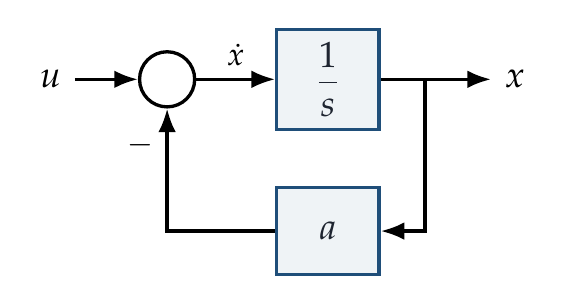
\begin{tikzpicture}[>={Latex[length=3mm]}, line width=1.2pt,
     blk/.style={draw, accent, fill=accent!7, minimum width=13mm, minimum height=11mm, font=\normalsize, text=ink},
     sum/.style={draw, circle, minimum size=7mm, inner sep=0pt, font=\small}]
    \node (u) {$u$};
    \node[sum, right=8mm of u] (s) {};
    \node[blk, right=10mm of s] (I) {$\dfrac1s$};
    \node[right=14mm of I] (y) {$x$};
    \node[blk, below=7mm of I] (a) {$a$};
    \draw[->] (u) -- (s);
    \draw[->] (s) -- node[above, font=\small]{$\dot x$} (I);
    \draw[->] (I) -- coordinate[pos=0.4](p) (y);
    \draw[->] (p) |- (a);
    \draw[->] (a) -| node[left, font=\small, pos=0.85]{$-$} (s);
  \end{tikzpicture}\\[1mm]
  {\small\color{muted}Each integrator holds one state: $\dot x=u-ax$, i.e.\ $\frac{1}{s+a}$.}}
\tcblower
\trap{Moving a summing junction past $G$ puts a copy of $G$ on \emph{every} branch through it. A cancelled pole is not gone, only hidden ($\lambda_7$).}
\end{mode}
\end{minipage}

\vspace{3mm plus 1fill}

\noindent\begin{minipage}[t]{0.488\linewidth}
\begin{mode}[equal height group=row5]{9}{Linearization}{Every curve is straight up close.}{Unlocks: small-signal models, operating points, predator--prey and epidemic thresholds, process control.}
\body[0.55]{%
  \begin{eqgroup}[Equilibrium first, then the Jacobians]
  \[ \mathbf f(\x_e,\uu_e)=\mathbf 0\qquad \delta\dot\x=\A\,\delta\x+\B\,\delta\uu \]
  \[ \A=\frac{\partial\mathbf f}{\partial\x}\Big|_e\quad \B=\frac{\partial\mathbf f}{\partial\uu}\Big|_e\quad
     \Cm=\frac{\partial\mathbf g}{\partial\x}\Big|_e\quad \D=\frac{\partial\mathbf g}{\partial\uu}\Big|_e \]
  \end{eqgroup}
  \begin{eqgroup}[It is only Taylor, cut after the slope]
  \[ f(x)\approx f(x_0)+f'(x_0)(x-x_0)\quad \text{error}\sim(x-x_0)^2 \]
  \end{eqgroup}
  \begin{eqgroup}[Three worked operating points]
  \[ \text{diode: } r_d=\frac{V_T}{I_D}\qquad \text{leaf spring: } k_{\text{eff}}=k_1+3k_2x_e^2 \]
  \[ \text{SIR: an outbreak dies out iff } R_0=\frac{\beta N}{\gamma}<1 \]
  \end{eqgroup}}%
{%
  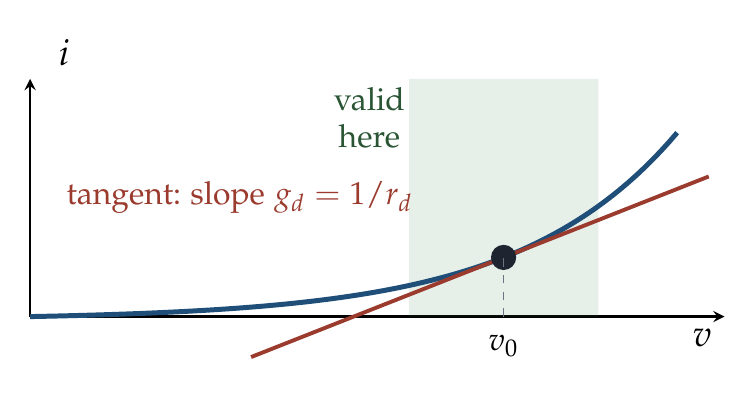
\begin{tikzpicture}
  \begin{axis}[posterplot, width=104mm, height=46mm, clip=false, axis lines=left, xmin=0, xmax=4.4, ymin=0, ymax=4.6,
      xlabel={$v$}, ylabel={$i$}, xtick={3}, xticklabels={$v_0$}, ytick=\empty,
      every axis y label/.style={at={(axis description cs:0,1)}, anchor=south west, xshift=2mm},
      every axis x label/.style={at={(axis description cs:1,0)}, anchor=north east}]
    \addplot[draw=none, fill=good, fill opacity=0.12] coordinates {(2.4,0) (3.6,0) (3.6,4.6) (2.4,4.6)} \closedcycle;
    \addplot[accent, domain=0:4.1, samples=80] {0.06*(exp(x)-1)};
    \addplot[trap, domain=1.4:4.3, samples=2, line width=1.4pt] {0.06*(exp(3)-1)+0.06*exp(3)*(x-3)};
    \fill[ink] (axis cs:3,{0.06*(exp(3)-1)}) circle (1.6mm);
    \draw[muted, dashed, thin] (axis cs:3,0) -- (axis cs:3,{0.06*(exp(3)-1)});
    \node[good!70!black, font=\small, align=center] at (axis cs:2.15,3.85) {valid\\here};
    \node[trap, font=\small, anchor=west, align=left] at (axis cs:0.15,2.3) {tangent:\ slope $g_d=1/r_d$};
  \end{axis}
  \end{tikzpicture}\\[1mm]
  {\small\color{muted}Shockley's diode, $i=I_s(e^{v/V_T}-1)$, near its bias point: a resistor $r_d\approx25\,\text{mV}/I_D$. Locally, $\operatorname{eig}\A$ decides stability (Hartman--Grobman).}}
\tcblower
\trap{When $\operatorname{eig}\A$ lands on the imaginary axis, the linearization is silent: Lotka--Volterra gives $\pm j\sqrt{\alpha\gamma}$, yet closed orbits. Saturation, hysteresis, chaos: lost.}
\end{mode}
\end{minipage}\hfill%
\begin{minipage}[t]{0.488\linewidth}
\begin{mode}[equal height group=row5]{10}{Discrete}{The unit circle is the new axis.}{Unlocks: digital control and DSP, simulation, Markov chains, Samuelson's economy, even tank battles.}
\body[0.54]{%
  \begin{eqgroup}[State equations and their solution]
  \[ \x[k+1]=\A\x[k]+\B\uu[k] \]
  \[ \x[k]=\A^k\x[0]+\sum_{i=0}^{k-1}\A^{k-1-i}\B\uu[i] \]
  \end{eqgroup}
  \begin{eqgroup}[$\A^k$: the same methods, $\lambda^k$ for $e^{\lambda t}$]
  \[ \A^k=\mathcal Z^{-1}\big\{z(z\I-\A)^{-1}\big\}=\V\Lam^k\V^{-1} \]
  \note{A Jordan block brings $k\lambda^{k-1}$ in place of $te^{\lambda t}$. Unlike $\Phi(t)$, $\A^k$ need not be invertible.}
  \end{eqgroup}
  \begin{eqgroup}[Sampling with a zero-order hold]
  \[ \A_D=e^{\A_cT}\qquad \B_D=(\A_D-\I)\A_c^{-1}\B_c \]
  \[ \text{Euler: }\A_D\approx\I+T\A_c\qquad z_i=e^{s_iT} \]
  \end{eqgroup}}%
{%
  {\eqsize $|\lambda_i|<1\ \forall i\iff$ asymptotically stable}\\[1mm]
  {\small\color{muted}$H(z)=\Cm(z\I-\A)^{-1}\B+\D$; $\ctrb$, $\obsv$ and block algebra unchanged.}\\[2mm]
  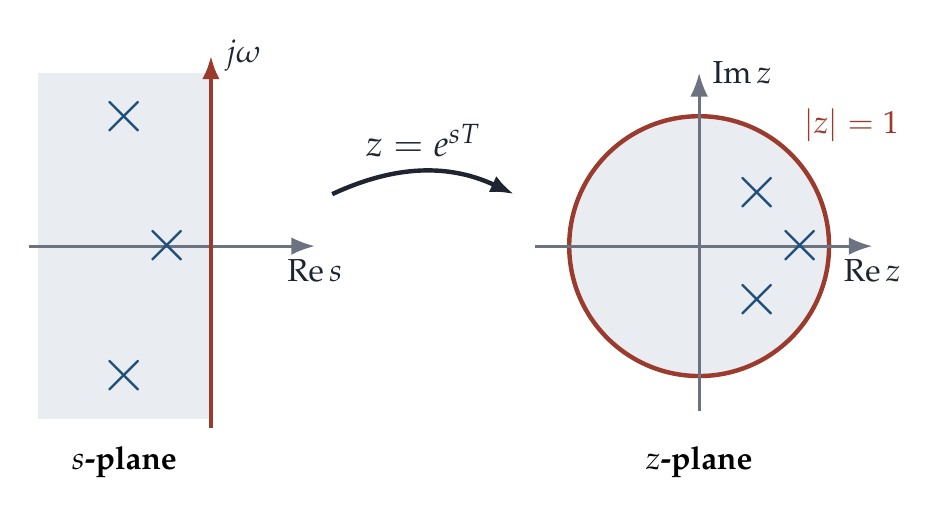
\begin{tikzpicture}[x=11mm, y=11mm, >={Latex[length=3mm]}]
    % s-plane
    \begin{scope}
      \fill[accent!10] (-2,-2) rectangle (0,2);
      \draw[->, muted, line width=1pt] (-2.1,0) -- (1.2,0) node[below, text=ink, font=\small]{$\operatorname{Re}s$};
      \draw[->, trap, line width=1.6pt] (0,-2.1) -- (0,2.2) node[right, text=ink, font=\small]{$j\omega$};
      \foreach \p/\q in {-1/1.5,-1/-1.5,-0.5/0}
        \node[accent, font=\fontsize{22}{22}\selectfont] at (\p,\q) {$\times$};
      \node[font=\small\bfseries] at (-1,-2.5) {$s$-plane};
    \end{scope}
    \draw[->, line width=1.6pt, ink] (1.4,0.6) to[bend left=25] node[above, font=\normalsize]{$z=e^{sT}$} (3.5,0.6);
    % z-plane
    \begin{scope}[xshift=62mm]
      \fill[accent!10] (0,0) circle (1.5);
      \draw[trap, line width=1.6pt] (0,0) circle (1.5);
      \draw[->, muted, line width=1pt] (-1.9,0) -- (2.0,0) node[below, text=ink, font=\small]{$\operatorname{Re}z$};
      \draw[->, muted, line width=1pt] (0,-1.9) -- (0,2.0) node[right, text=ink, font=\small]{$\operatorname{Im}z$};
      \foreach \p/\q in {0.666/0.62,0.666/-0.62,1.168/0}
        \node[accent, font=\fontsize{22}{22}\selectfont] at (\p,\q) {$\times$};
      \node[trap, font=\small, anchor=south west] at (1.06,1.06) {$|z|=1$};
      \node[font=\small\bfseries] at (0,-2.5) {$z$-plane};
    \end{scope}
  \end{tikzpicture}\\[2mm]
  {\small\color{muted}The left half-plane folds into the unit disc, the $j\omega$ axis onto the circle. With ZOH, $|z_i|=e^{\operatorname{Re}s_i\,T}$: stability never depends on $T$. Euler's $z_i=1+Ts_i$ can leave the disc if $T$ is too large.}}
\tcblower
\trap{Every $Z$ pair carries a $z$ on top ($a^k\leftrightarrow\frac{z}{z-a}$): expand $\frac{Y(z)}{z}$, then multiply back by $z$. There is no pair for $\frac{K}{z-a}$ alone: it is a delayed $a^{k-1}$.}
\end{mode}
\end{minipage}

\end{document}
